\documentclass[border=0.125cm]{standalone}
\usepackage{tikz}
\usetikzlibrary{matrix}

\begin{document}
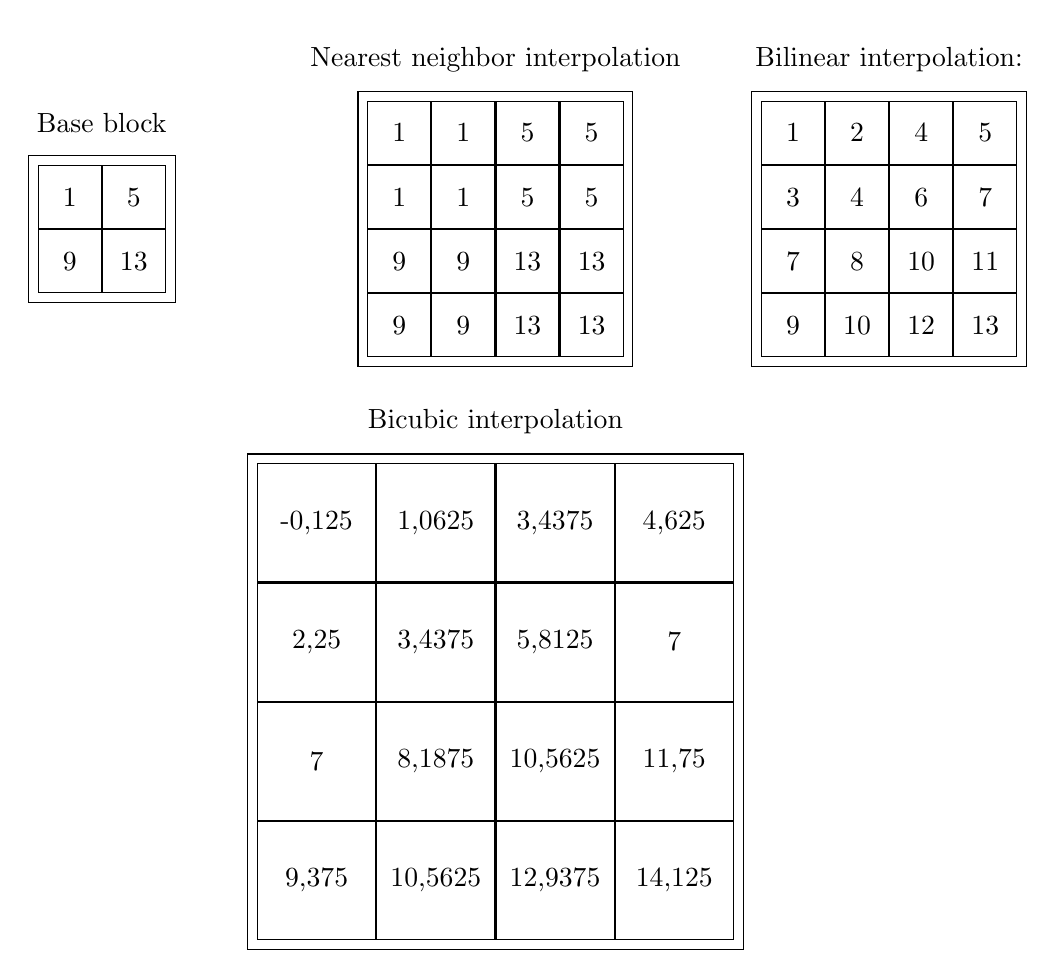
\begin{tikzpicture}
\tikzstyle{every node}=[draw, minimum size=0.8cm]
\matrix [draw=black, label = {above:Base block}](ref) at (0,0)
{
	\node {1}; & \node{5}; \\
	\node {9}; & \node{13}; \\
};
\matrix [draw=black, label = {above:Nearest neighbor interpolation}](near) at (5,0){Nearest neighbor}
{
	\node {1}; & \node{1}; & \node {5}; & \node {5}; \\
	\node {1}; & \node{1}; & \node {5}; & \node {5}; \\
	\node {9}; & \node{9}; & \node {13}; & \node {13}; \\
	\node {9}; & \node{9}; & \node {13}; & \node {13};\\
};
\matrix [draw=black, label = {above:Bilinear interpolation:}](bil) at (10,0)
{
	\node {1}; & \node{2}; & \node {4}; & \node {5}; \\
	\node {3}; & \node{4}; & \node {6}; & \node {7}; \\
	\node {7}; & \node{8}; & \node {10}; & \node {11}; \\
	\node {9}; & \node{10}; & \node {12}; & \node {13}; \\
};
\matrix [draw=black, nodes={minimum size = 1.5cm}, label = {above:Bicubic interpolation}](bic) at (5,-6)
{
	\node {-0,125}; & \node{1,0625}; & \node {3,4375}; & \node {4,625}; \\
	\node {2,25}; & \node{3,4375}; & \node {5,8125}; & \node {7}; \\
	\node {7}; & \node{8,1875}; & \node {10,5625}; & \node {11,75}; \\
	\node {9,375}; & \node{10,5625}; & \node {12,9375}; & \node {14,125}; \\
};
%\node[anchor=south] at (ref.north) {Base block:};
%\node[anchor=south] at (near.north) {Nearest neighbor:};
%\node[anchor=south] at (bil.north) {Bilinear:};
%\node[anchor=south] at (bic.north) {Bicubic:};
\end{tikzpicture}
\end{document}